% Appendix Template

\chapter{Preliminary Definition} % Main appendix title

\label{AppendixDef} % Change X to a consecutive letter; for referencing this appendix elsewhere, use \ref{AppendixX}

\lhead{\chaptername~\thechapter. \emph{Preliminary Definition}} % Change X to a consecutive letter; this is for the header on each page - perhaps a shortened title

%----------------------------------------------------------------------------------------
%    Preamble
%----------------------------------------------------------------------------------------

\section{Preamble}
\label{sec:def_preamble}

%----------------------------------------------------------------------------------------
%    Paper Description
%----------------------------------------------------------------------------------------

\section{Paper Description}
\label{sec:def_paper_description}

% \makeatletter
% 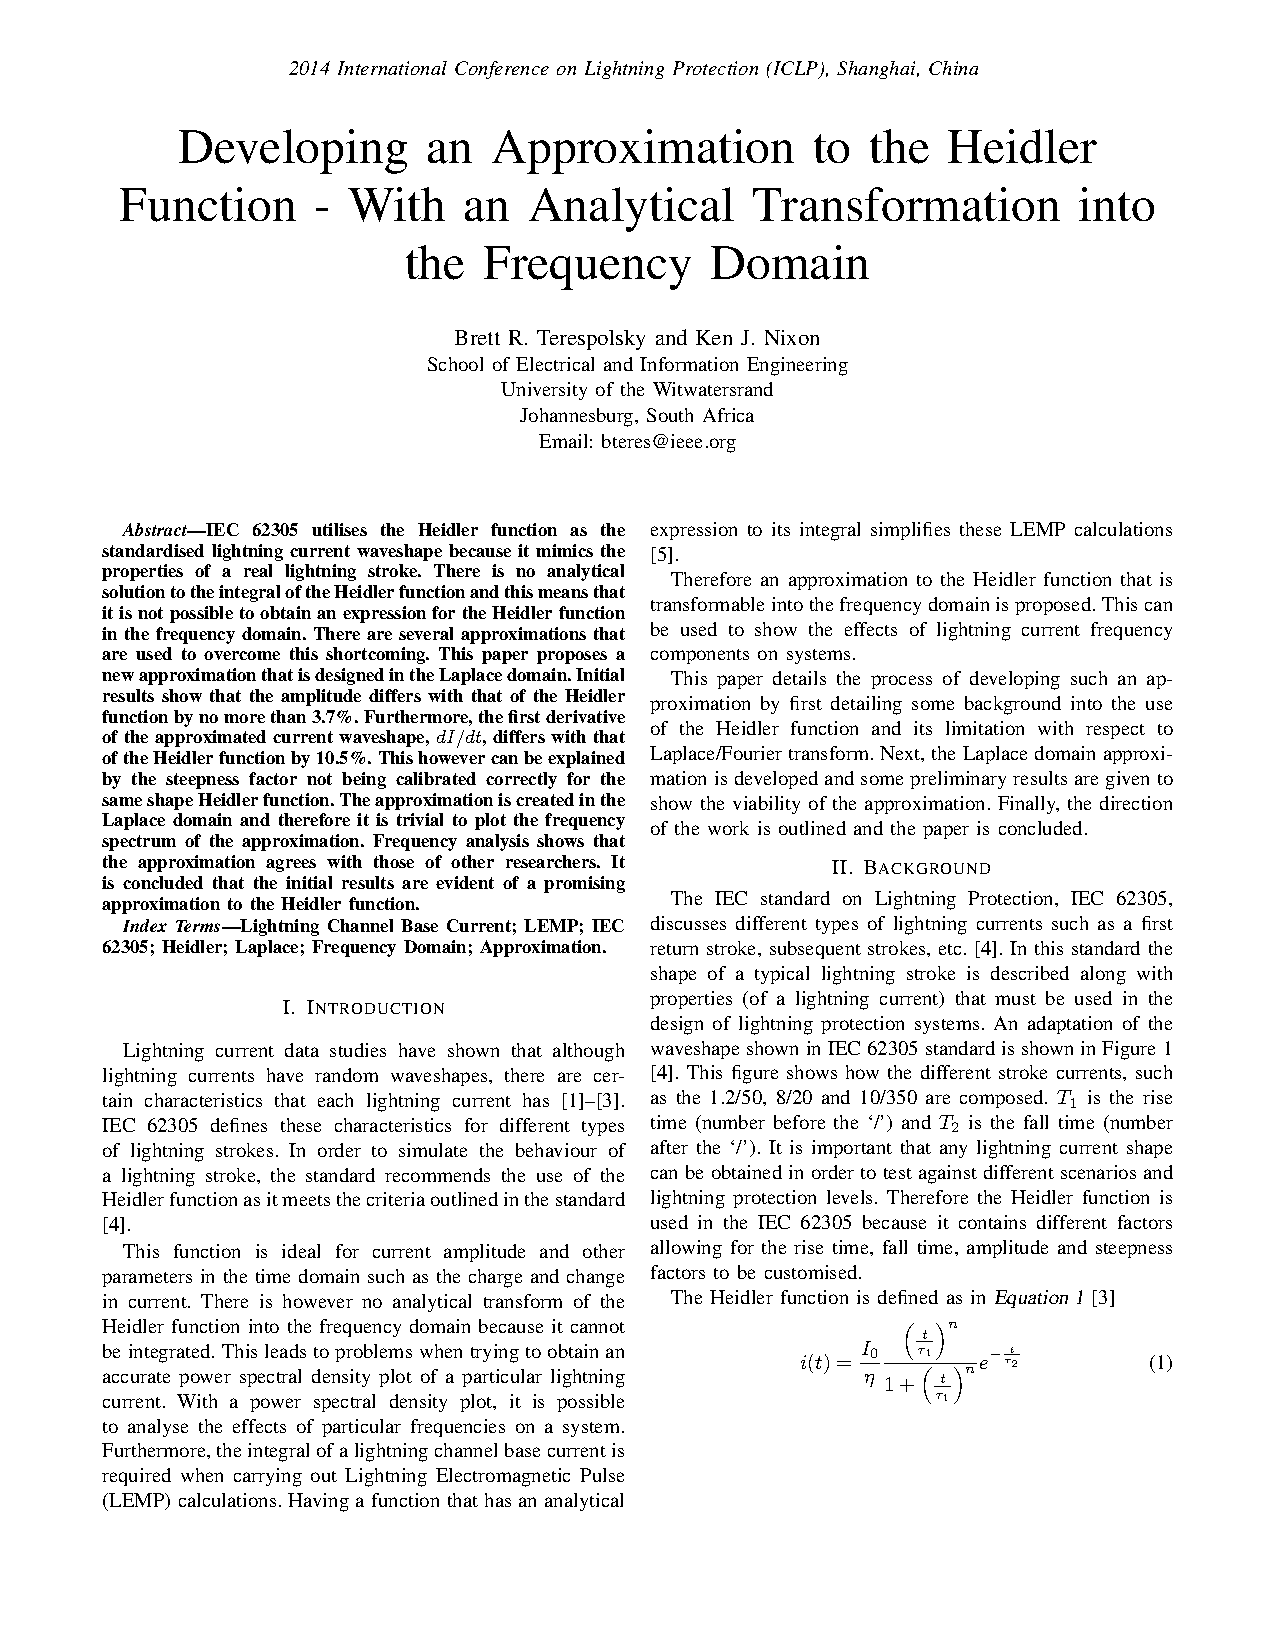
\includepdf[
%   pages=-,
%   width=\Gm@layoutwidth,
%   height=\Gm@layoutheight,
%   offset={\dimexpr(\Gm@layoutwidth-\paperwidth)/2\relax}
%          {\dimexpr(\paperheight-\Gm@layoutheight)/2\relax},
%   keepaspectratio=true
%   ]{./AdditionalFiles/BrettTerespolskyICLP2014}
% \makeatother

% 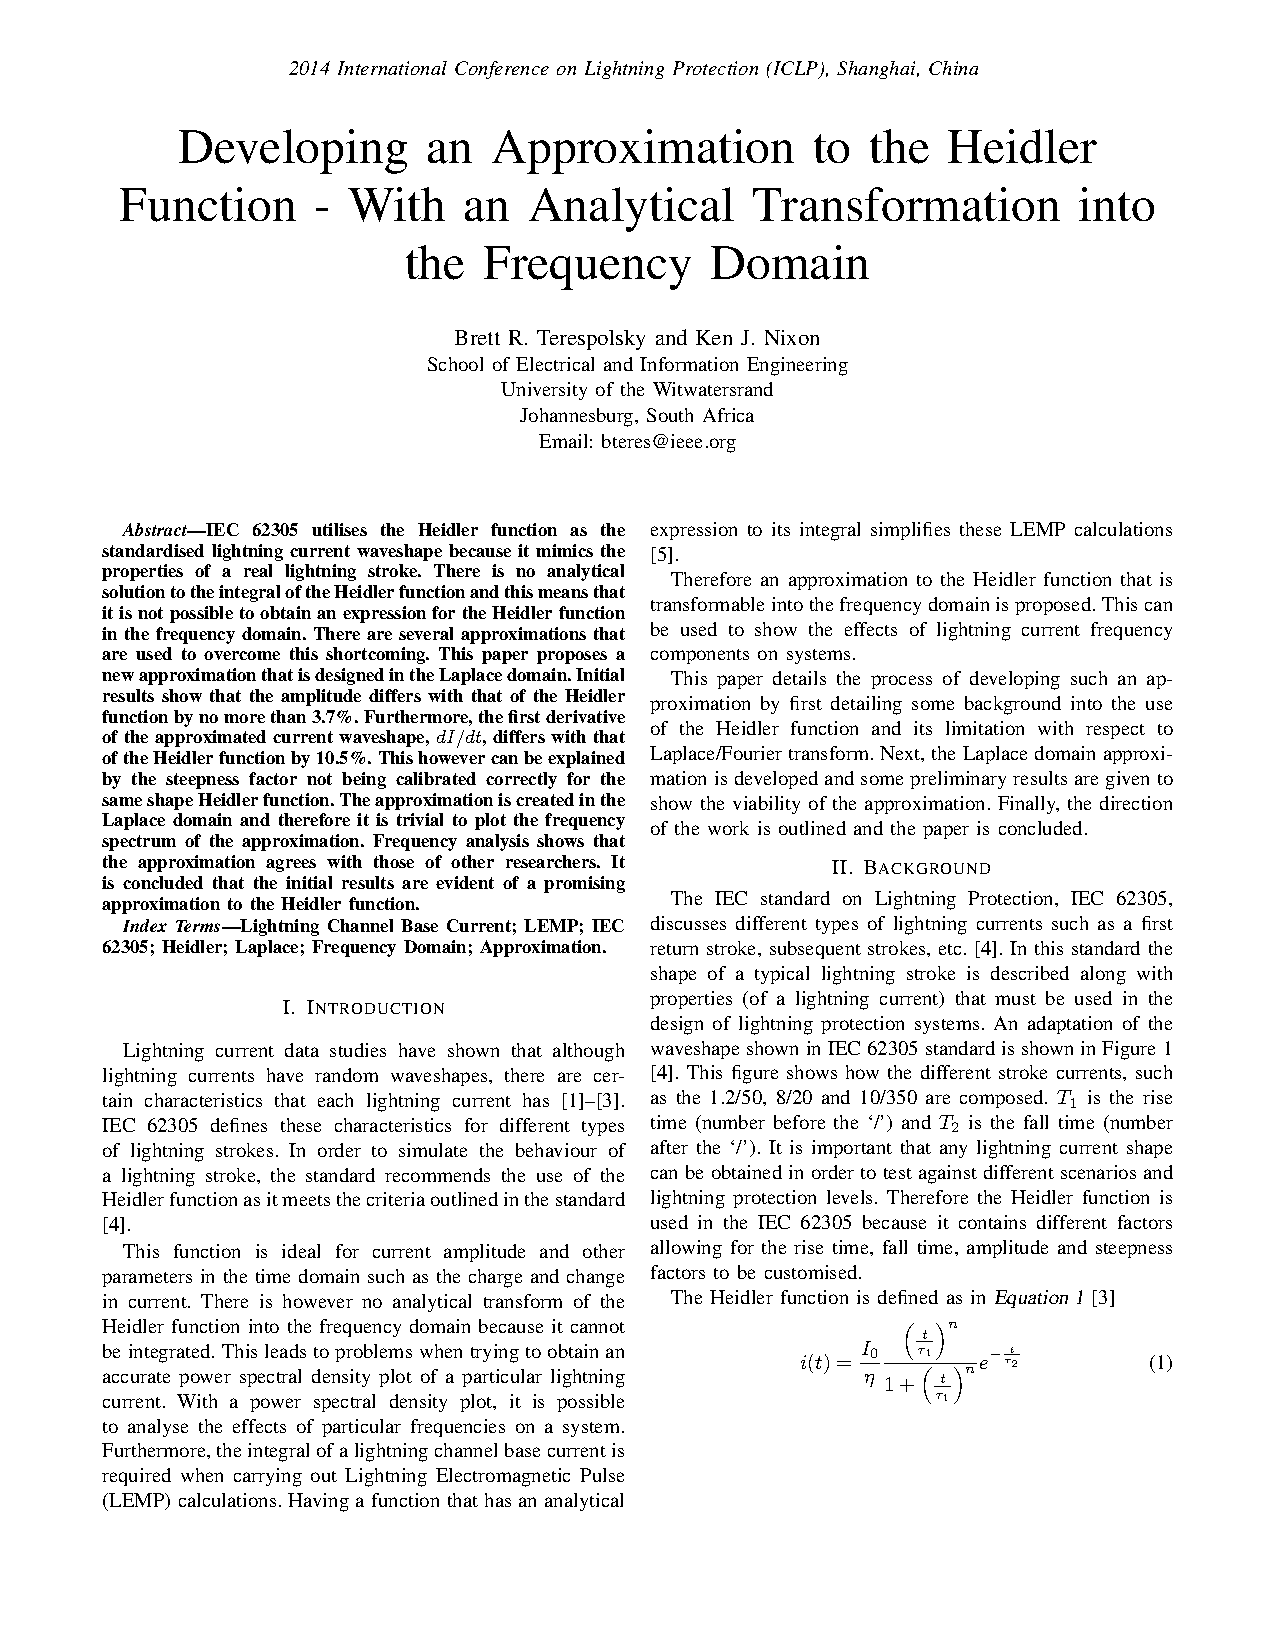
\includepdf[
%   % width=\linewidth,
%   % keepaspectratio=true
%   ]{./AdditionalFiles/BrettTerespolskyICLP2014}
